\begin{figure*}[t]
    \centering
    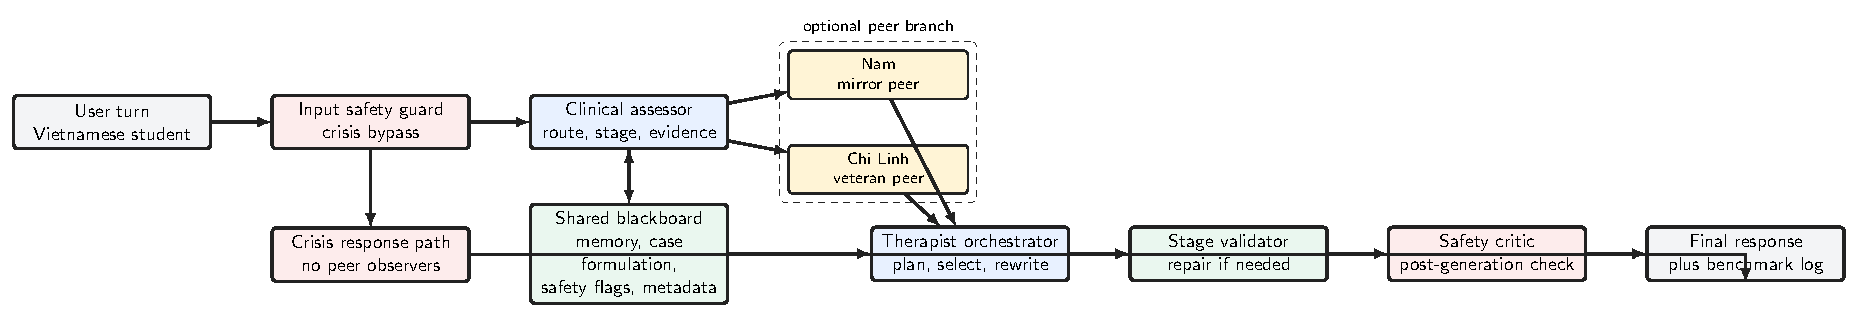
\includegraphics[width=0.94\linewidth]{figures/system_architecture.pdf}
    \caption{\trace\ process-controlled dialogue graph. The blackboard stores route, stage, evidence, safety flags, case formulation, peer policy, and metadata; peer agents are optional and gated before final response generation.}
    \label{fig:system_architecture}
\end{figure*}

\subsection{Problem Setting and Design Goals}
We target support-oriented Vietnamese student dialogue, not diagnosis, treatment, crisis service, or clinical deployment. \trace\ must respond to academic and interpersonal distress while preserving route-specific process. The key design choice is to make process state explicit: validating distress, eliciting an automatic thought, planning a behavioral activation step, guiding a mindfulness exercise, and handling a safety boundary are different actions, even if all can be phrased empathically.

Figure~\ref{fig:system_architecture} gives the full flow. A user turn first passes through onboarding and safety checks, then updates a shared blackboard through an assessor. Optional peer agents generate short support drafts, and the therapist orchestrator decides whether these drafts should be included, rewritten, or discarded. Validator and safety modules then repair or replace the final response when required.

The architecture is designed around five goals: preserve a single support route within a turn, pace stage transitions through explicit evidence, use peer voices only when they serve a narrow group-support function, expose safety and fallback behavior in metadata, and support ablation experiments without changing the benchmark interface. Table~\ref{tab:vsm_capabilities} summarizes how the main VSM capabilities map to \trace\ mechanisms.

\begin{table}[t]
\centering
\footnotesize
\setlength{\tabcolsep}{3pt}
\begin{tabular}{p{0.28\linewidth}p{0.62\linewidth}}
\toprule
Capability & System mechanism \\
\midrule
Route fidelity & Assessor updates route evidence in the blackboard and records route metadata for scoring. \\
Stage fidelity & Dynamic formulation plus milestone FSM controls support-stage progression. \\
Technique fidelity & Therapist orchestrator and validator align the response with the current route/stage task. \\
Peer dynamics & Yalom-factor gating decides whether Nam, Linh, or no peer may contribute. \\
Safety & Crisis bypass and post-generation safety critic block unsafe support patterns. \\
Auditability & Shared blackboard emits route, stage, peer, validator, safety, fallback, and latency fields. \\
\bottomrule
\end{tabular}
\caption{Target VSM capabilities and the corresponding mechanisms in the full system.}
\label{tab:vsm_capabilities}
\end{table}


\subsection{Dynamic Blackboard Formulation}
The central representation is a typed blackboard state shared by all nodes. It functions as a lightweight dynamic formulation: an internal state object that makes process decisions explicit without claiming to be a clinical diagnosis. For each turn, the blackboard stores the user message, history, selected model, system variant, active route, current stage, route-specific evidence, case-formulation fields, safety flags, peer drafts, therapist plan, validator status, fallback status, latency, and final response.

\begin{figure}[t]
    \centering
    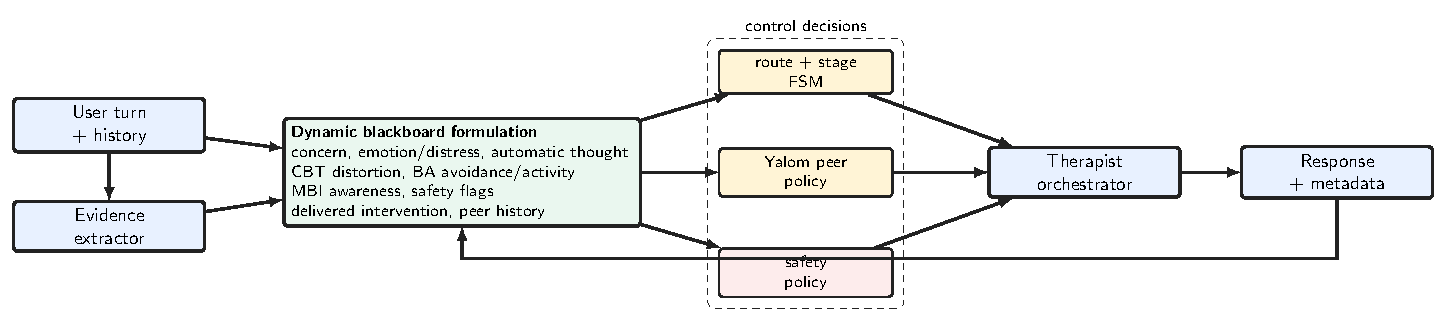
\includegraphics[width=\linewidth]{figures/case_formulation_blackboard.pdf}
    \caption{Dynamic blackboard formulation. User evidence updates a shared state, which then controls route/stage progression, peer gating, safety policy, response generation, and benchmark metadata.}
    \label{fig:case_formulation_blackboard}
\end{figure}

Figure~\ref{fig:case_formulation_blackboard} shows the control role of this state. The formulation includes presenting concern, emotion and distress, automatic thought or belief, CBT distortion evidence, BA avoidance or activity evidence, MBI awareness evidence, peer boundary intent, safety flags, delivered therapist intervention, and peer history or cooldown. The design is inspired by CBT case formulation but is deliberately broader: it is optimized for multi-route control and benchmark audit rather than reconstructing a full clinical conceptualization diagram. The same schema makes ablations comparable, because every variant emits route, stage, peer, validator, safety, fallback, and latency fields even when a mechanism is disabled.

\subsection{Evidence Extraction and Stage Control}
The clinical assessor updates the blackboard before generation. For CBT, it extracts structured evidence such as event, emotion, automatic thought, distortion reflection, Socratic reasoning, balanced reframe, action commitment, overload, and peer-boundary intent. A deterministic milestone controller then chooses the stage; the extractor is not allowed to directly set the stage. For BA and MBI, route-specific evidence extractors feed deterministic stage detectors.

\begin{algorithm}[t]
\small
\caption{Stage-Aware Blackboard Update}
\label{alg:blackboard_update}
\begin{algorithmic}[1]
\Require user turn $u_t$, history $H_t$, previous blackboard $B_{t-1}$
\Ensure updated blackboard $B_t$
\State $S \gets$ safety\_input\_check($u_t$, $H_t$)
\If{$S$ indicates crisis}
    \State set route to \textsc{crisis}; disable peer observers
    \State \Return crisis blackboard update
\EndIf
\State $r \gets$ active route from onboarding/protocol state
\State $E \gets$ extract route-specific evidence($u_t$, $H_t$, $r$)
\State $M \gets$ update milestone state($B_{t-1}$, $E$, delivered interventions)
\State $s_t \gets$ deterministic stage controller($r$, $M$, $B_{t-1}$)
\State $Y_t \gets$ required Yalom factors($r$, $s_t$, $E$)
\State \Return $B_t$ with route, stage, evidence, milestones, safety, and peer policy
\end{algorithmic}
\end{algorithm}

\begin{figure}[t]
    \centering
    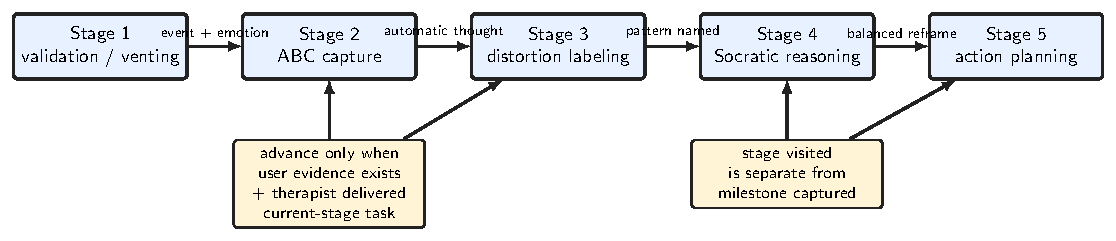
\includegraphics[width=\linewidth]{figures/stage_state_machine.pdf}
    \caption{CBT stage pacing. Progression requires both user-side evidence and prior therapist intervention, preventing a single strong user message from skipping intermediate stages.}
    \label{fig:stage_state_machine}
\end{figure}

Figure~\ref{fig:stage_state_machine} shows the CBT controller. The system distinguishes milestones observed in the user message from stages already visited by the therapist. A transition requires both user-side evidence and evidence that the therapist has delivered the current-stage intervention. For example, an action phrase does not immediately move the system to action planning if ABC or Socratic work has not been delivered. This rule is the main process-control difference between the proposed graph and a single prompt that simply reacts to the newest user message.

\subsection{Therapist Orchestrator}
The therapist orchestrator reads route, stage, case formulation, safety report, clinical knowledge, required Yalom factors, and peer drafts. It returns a structured plan and the therapist message. The orchestrator may include, rewrite, or discard peer drafts, but the final inclusion is checked again by route and persona policy. If the therapist message misses the stage goal, the validator can repair it with a stage-specific fallback. This keeps the peer branch subordinate to therapist-led process rather than allowing independent agents to steer the session.

\subsection{Yalom-Factor Peer Gating}
The full system includes two peer personas. Nam is a mirror peer for brief universality or catharsis; he should not perform therapist techniques or give advice. Linh is a veteran peer for hope or interpersonal learning; she should not dominate the turn or provide directive advice. Peer use is controlled by route, stage, required Yalom factor, safety status, user boundary intent, and cooldown.

\begin{figure}[t]
    \centering
    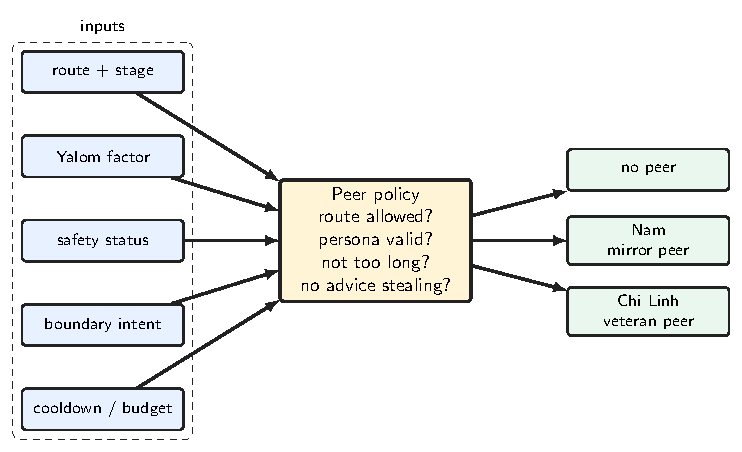
\includegraphics[width=\linewidth]{figures/peer_gating.pdf}
    \caption{Peer gating contract. The output is either no peer, mirror peer, or veteran peer; no-peer and single-agent variants report peer absence explicitly.}
    \label{fig:peer_gating}
\end{figure}

This contract prevents peer agents from appearing in stages where therapist-led work should remain focused. CBT Socratic questioning, for instance, silences peers by policy. When the user signals that peer input is distracting, the assessor sets a boundary field and the required Yalom factor becomes \texttt{NONE}.

\begin{algorithm}[t]
\small
\caption{Peer Gating and Response Finalization}
\label{alg:peer_response}
\begin{algorithmic}[1]
\Require blackboard $B_t$, peer drafts $P_t$, therapist draft $d_t$
\Ensure final response $R_t$ and benchmark metadata
\State $P'_t \gets$ filter drafts by route, stage, Yalom factor, safety, and cooldown
\State $D_t \gets$ orchestrator decisions over $P'_t$ and $d_t$
\State $R_t \gets$ include, rewrite, or discard peer drafts according to $D_t$
\If{validator is enabled and therapist message misses stage goal}
    \State repair therapist message with a stage-specific fallback
\EndIf
\If{safety critic is enabled and combined output is high-risk}
    \State replace response with safety fallback; clear peer output
\EndIf
\State emit final response plus route, stage, peer, validator, safety, fallback, and latency metadata
\end{algorithmic}
\end{algorithm}

\subsection{Safety and Guardrails}
Safety handling occurs at multiple points. Safety-critical input can bypass peer dynamics and enter a crisis-oriented response path. During generation, the orchestrator receives a psychosocial safety report. After generation, the safety critic can replace the response with a safety fallback if the combined peer and therapist output is high-risk. The final guardrails node cleans unsafe advice, maps internal speaker IDs to user-facing names, packages \texttt{final\_reply}, and records safety metadata.

\subsection{Paper-Facing Variants}
The evaluation names the full graph \tracefull. Three ablations disable one mechanism while preserving the rest of the graph: \textsc{TRACE-NoPeer}, \textsc{TRACE-NoValidator}, and \textsc{TRACE-NoSafetyCritic}. The stage-prompt baseline receives route and stage but no peer planning or shared blackboard coordination. The plain baseline generates a supportive response without route, stage, or peer-control logic. All variants return a common result schema for final text, route, stage, peer, validator, safety, fallback, and latency fields, making differences attributable to system behavior rather than adapter-specific parsing.
